\section{The stripped BeTSSi submarine model}
\label{Sec2:BeTSSi_description}
In this section a simplified version of the BeTSSi submarine model (depicted in \Cref{Fig2:BeTSSi_BC}) will be presented. Namely a \textit{stripped BeTSSi submarine model} without sail and rudders as in \Cref{Fig2:BeTSSi_BC_stripped}.
\begin{figure}
	\centering
	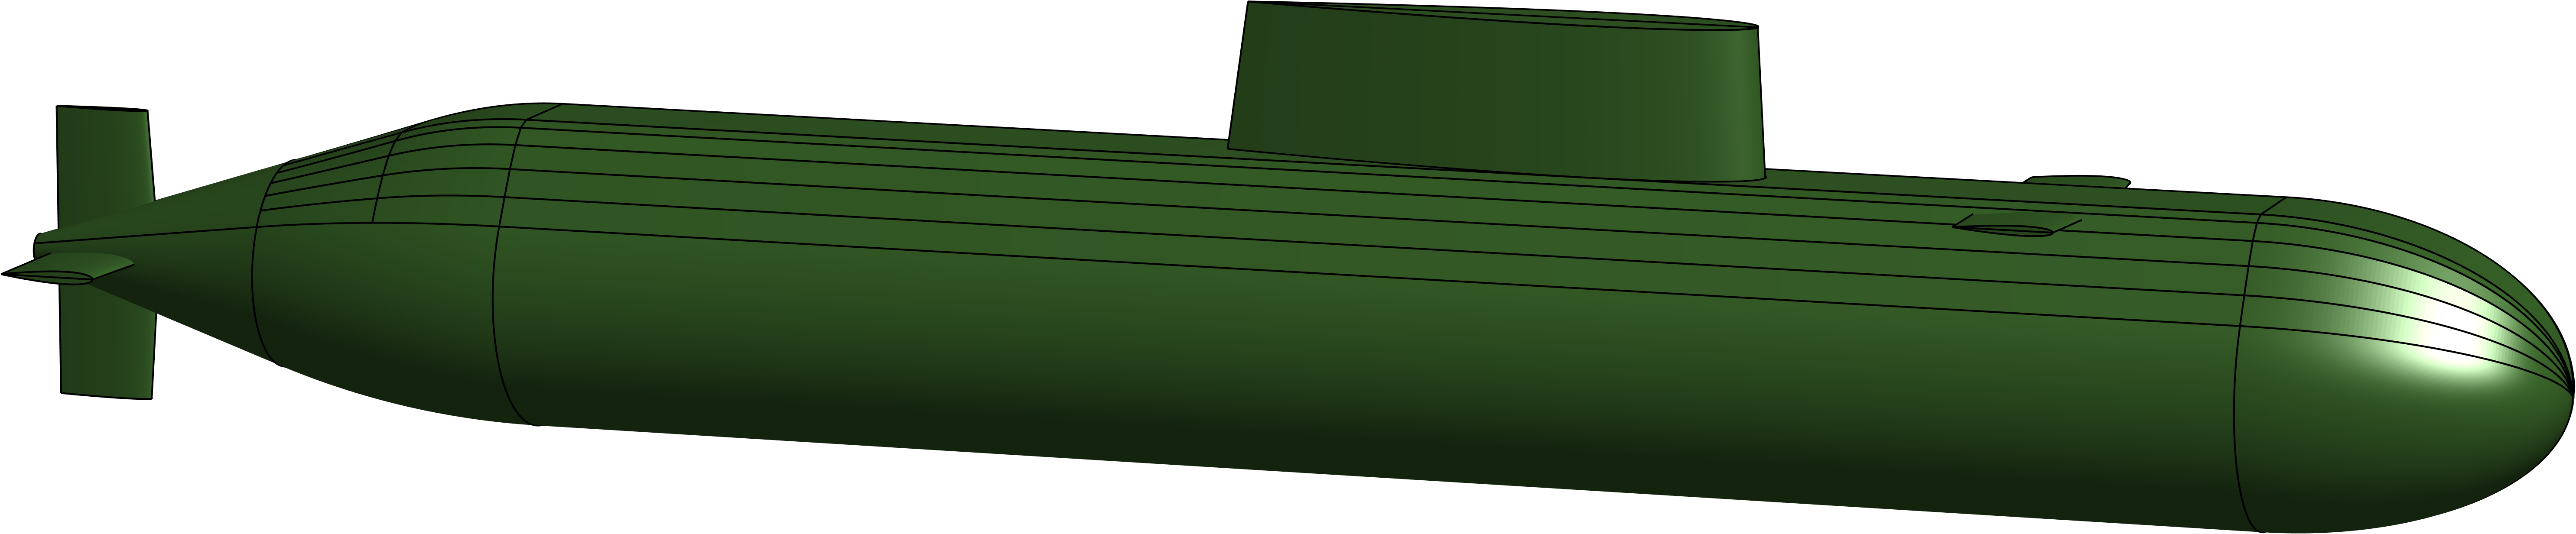
\includegraphics[width=\textwidth]{BeTSSi_BC}
	\caption{Outer pressure hull for BeTSSi submarine.}
	\label{Fig2:BeTSSi_BC}
\end{figure}
\begin{figure}
	\centering
	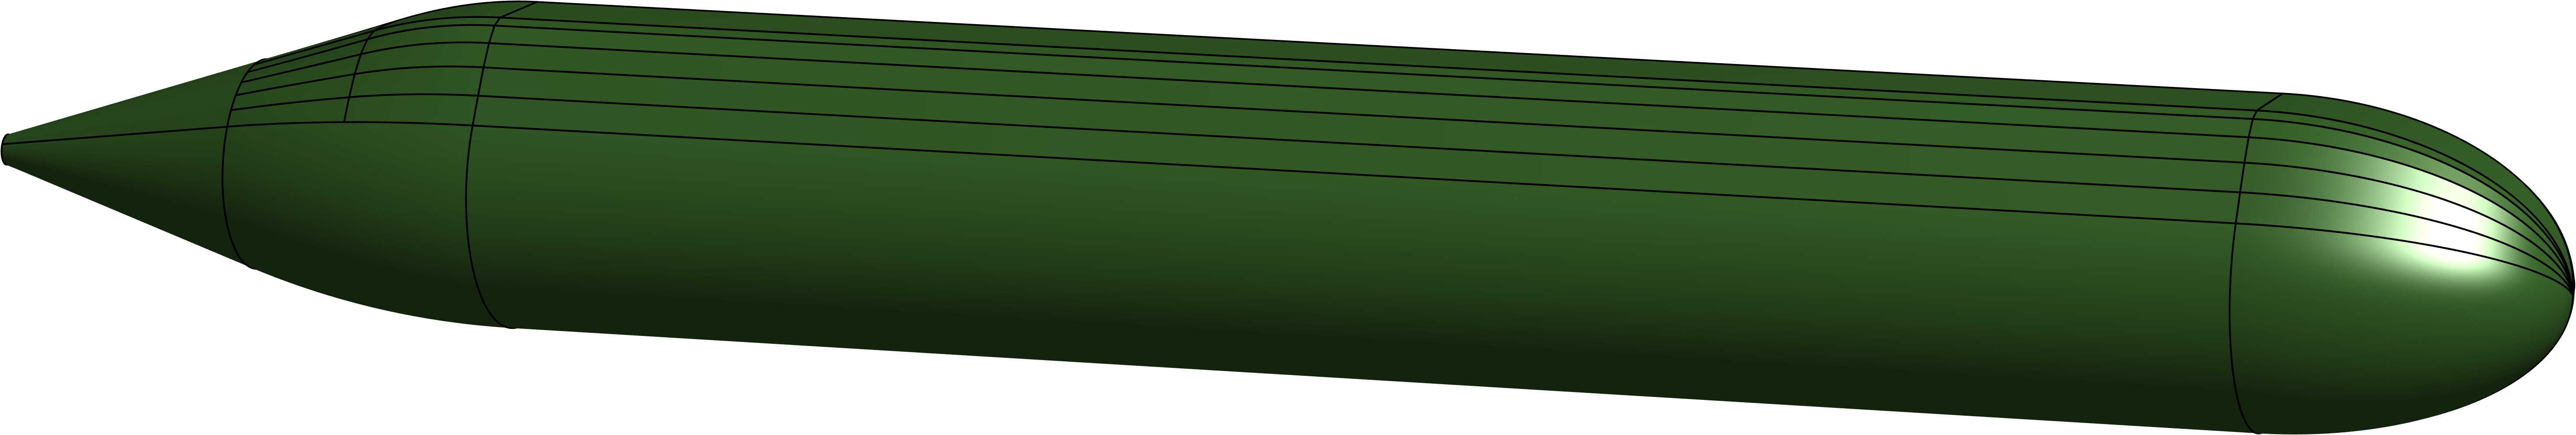
\includegraphics[width=\textwidth]{BeTSSi_BC_stripped}
	\caption{The stripped BeTSSi submarine model.}
	\label{Fig2:BeTSSi_BC_stripped}
\end{figure}
The relevant BeTSSi parameters for the work presented herein are given in \Cref{Tab2:BeTSSiParameters}.
\begin{table}
	\centering
	\caption{\textbf{BeTSSi submarine:} Parameters for the BeTSSi submarine benchmark.}
	\label{Tab2:BeTSSiParameters}
	\begin{tabular}{l l}
		\toprule
		Parameter & Description\\
		\midrule
		$P_{\mathrm{inc}}=\SI{1}{Pa}$ & Amplitude of incident wave\\
		$E = \SI{2.10e11}{Pa}$ & Young's modulus\\
		$\nu = 0.3$ & Poisson's ratio\\
		$\rho_{\mathrm{s}} = \SI{7850}{kg.m^{-3}}$ & Density of solid\\
		$\rho_{\mathrm{f}} = \SI{1000}{kg.m^{-3}}$ & Density of water\\
		$c_{\mathrm{f}} = \SI{1500}{m.s^{-1}}$ & Speed of sound in water\\
		$t=\SI{0.01}{m}$ & Thickness of pressure hull\\
		$\alpha=\ang{18}$ & Arc angle of transition to the tail cone\\
		$\beta=\ang{240}$ & Rotational angle for the axisymmetric lower part\\
		$g_2=\SI{6.5}{m}$ & Distance in $x$-direction of transition to the tail cone\\
		$g_3=\SI{6.5}{m}$ & Distance in $x$-direction of the tail cone\\
		$L=\SI{42}{m}$ & Length of the deck\\
		$a=\SI{7}{m}$ & Semi-major axis of bow\\
		$b=\SI{3.5}{m}$ & Semi-major axis of bow\\
		$c=\SI{4}{m}$ & Height from $x$-axis to the deck\\
		$s=\SI{1.2}{m}$ & Half of the width of the deck\\
		\bottomrule
	\end{tabular}
\end{table}
The model is symmetric about the $xz$-plane and has rotational symmetry for the lower part as described in \Cref{Fig2:bettsi_bottom}.
\begin{figure}
	\centering
	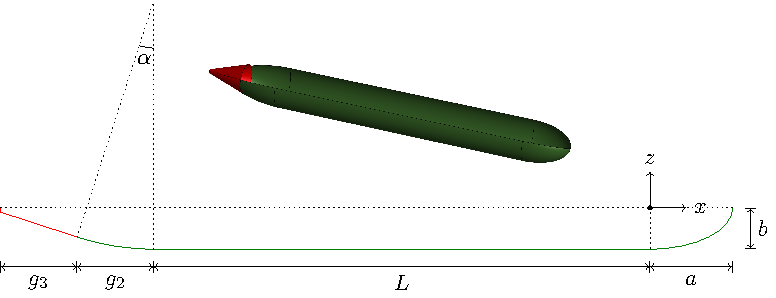
\includegraphics[scale=1]{betssi_bottom}
	\caption{The sideline of the lower part of the BeTSSi submarine. The sidelines are formed (from the right) by an ellipse with semi-major axis $a$ and semi-minor axis $b$, followed by a straight line of length $L$, then an arc of angle $\alpha$ and finally two straight lines. The latter two straight lines (in red) are rotated about the $x$-axis and the remaining part (in green) are rotated an angle $\beta$ around the $x$-axis.}
	\label{Fig2:bettsi_bottom}
\end{figure}
The transition from this axisymmetric part to the deck is described in \Cref{Fig2:bettsi_top}. This transition as well as the deck itself, contains a set of rectangular panels of length $L$.
\begin{figure}
	\centering
	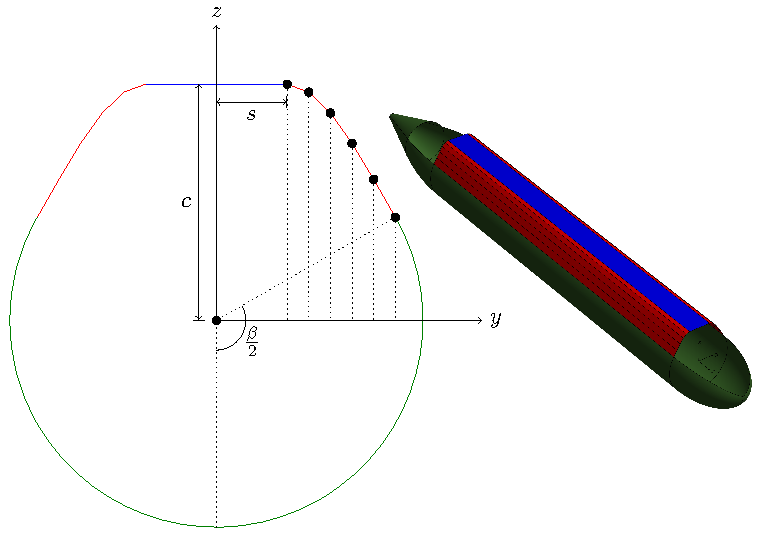
\includegraphics[scale=1]{betssi_top}
	\caption{The transition (red line) from the axisymmetric hull (green line) to the deck (blue line) is given by sampling a cubic polynomial, $P(y)$, at 6 equidistant points in the $y$-direction and connecting the resulting points with straight lines (corresponding 6 points are found for negative values $y$-values, $(0,y,P(|y|))$).}
	\label{Fig2:bettsi_top}
\end{figure}
The polynomial $P(y)$, is uniquely defined by the requirement that it defines a smooth transition between the hull and the deck. More precisely, the following requirement must be satisfied: 
\begin{alignat*}{3}
	P(s) &= c,\quad  &&P\left(b\sin\frac{\beta}{2}\right) = -b\cos\frac{\beta}{2}\\
	P'(s) &= 0,\quad &&P'\left(b\sin\frac{\beta}{2}\right) = \tan\frac{\beta}{2}
\end{alignat*}
which gives the polynomial
\begin{equation}
	P(y) = c+C_1(y-s)^2+C_2(y-s)^3
\end{equation}
where
\begin{align*}
	C_1 = -\frac{3C_4+C_3\tan\frac{\beta}{2}}{C_3^2}, \quad
	C_2 = \frac{2C_4+C_3\tan\frac{\beta}{2}}{C_3^3},\\
	C_3 = b\sin\frac{\beta}{2}-s, \quad
	C_4 = c+b\cos\frac{\beta}{2}.
\end{align*}
The upper part of the bow (highlighted in \Cref{Fig2:bettsi_upperBow}) is obtained by linear lofting of elliptic curves from the 12 points described in \Cref{Fig2:bettsi_top} to the tip of the bow. The upper part of the tail section (highlighted in \Cref{Fig2:bettsi_upperPartOfTailSection}) is connected using a tensor NURBS surface of degree 2 such that it defines a smooth transition from the axisymmetric cone to the deck. More precisely, the upper part of the cone tail is divided into 12 arcs with angle $\frac{2\PI-\beta}{12}$, and the resulting points are connected to corresponding points on the transition to the deck from the axisymmetric hull. 
\begin{figure}
	\centering    
	\begin{subfigure}{0.49\textwidth}
		\centering
		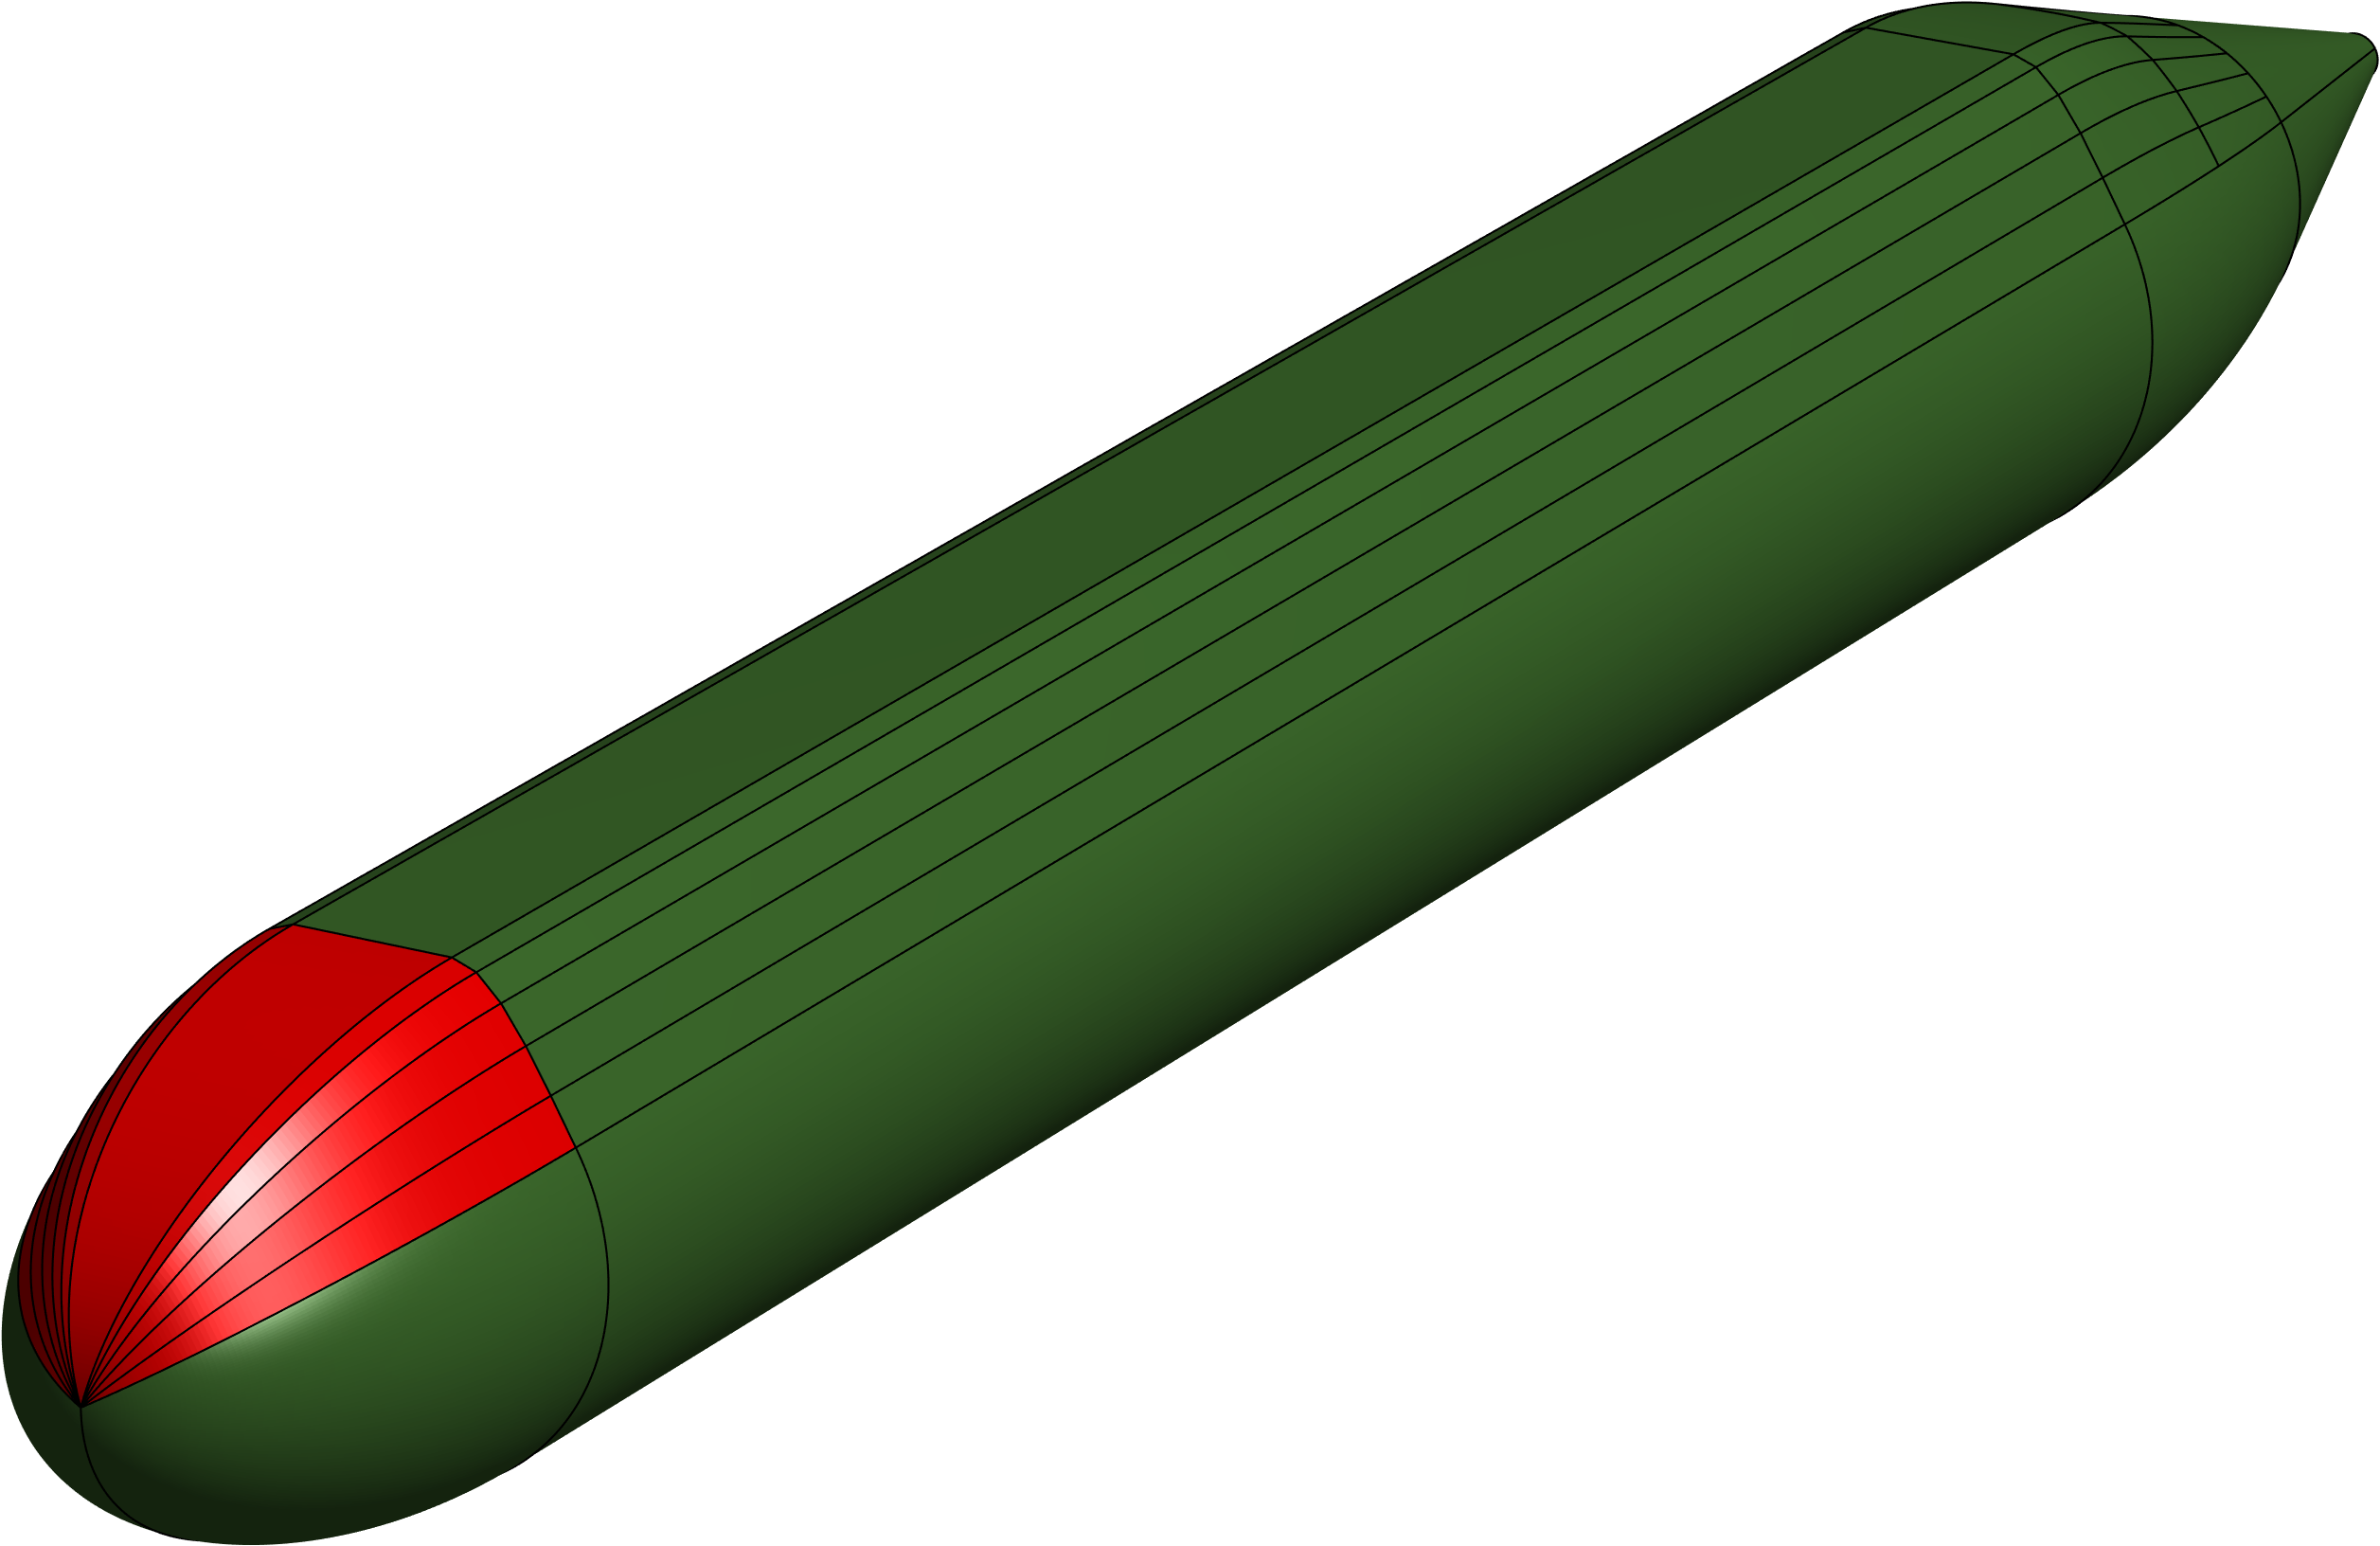
\includegraphics[width=\textwidth]{BeTSSi_BCpart4}
		\caption{Illustration of upper bow part.}
		\label{Fig2:bettsi_upperBow}
	\end{subfigure}%
	\hspace*{0.02\textwidth}%   
	\begin{subfigure}{0.49\textwidth}
		\centering
		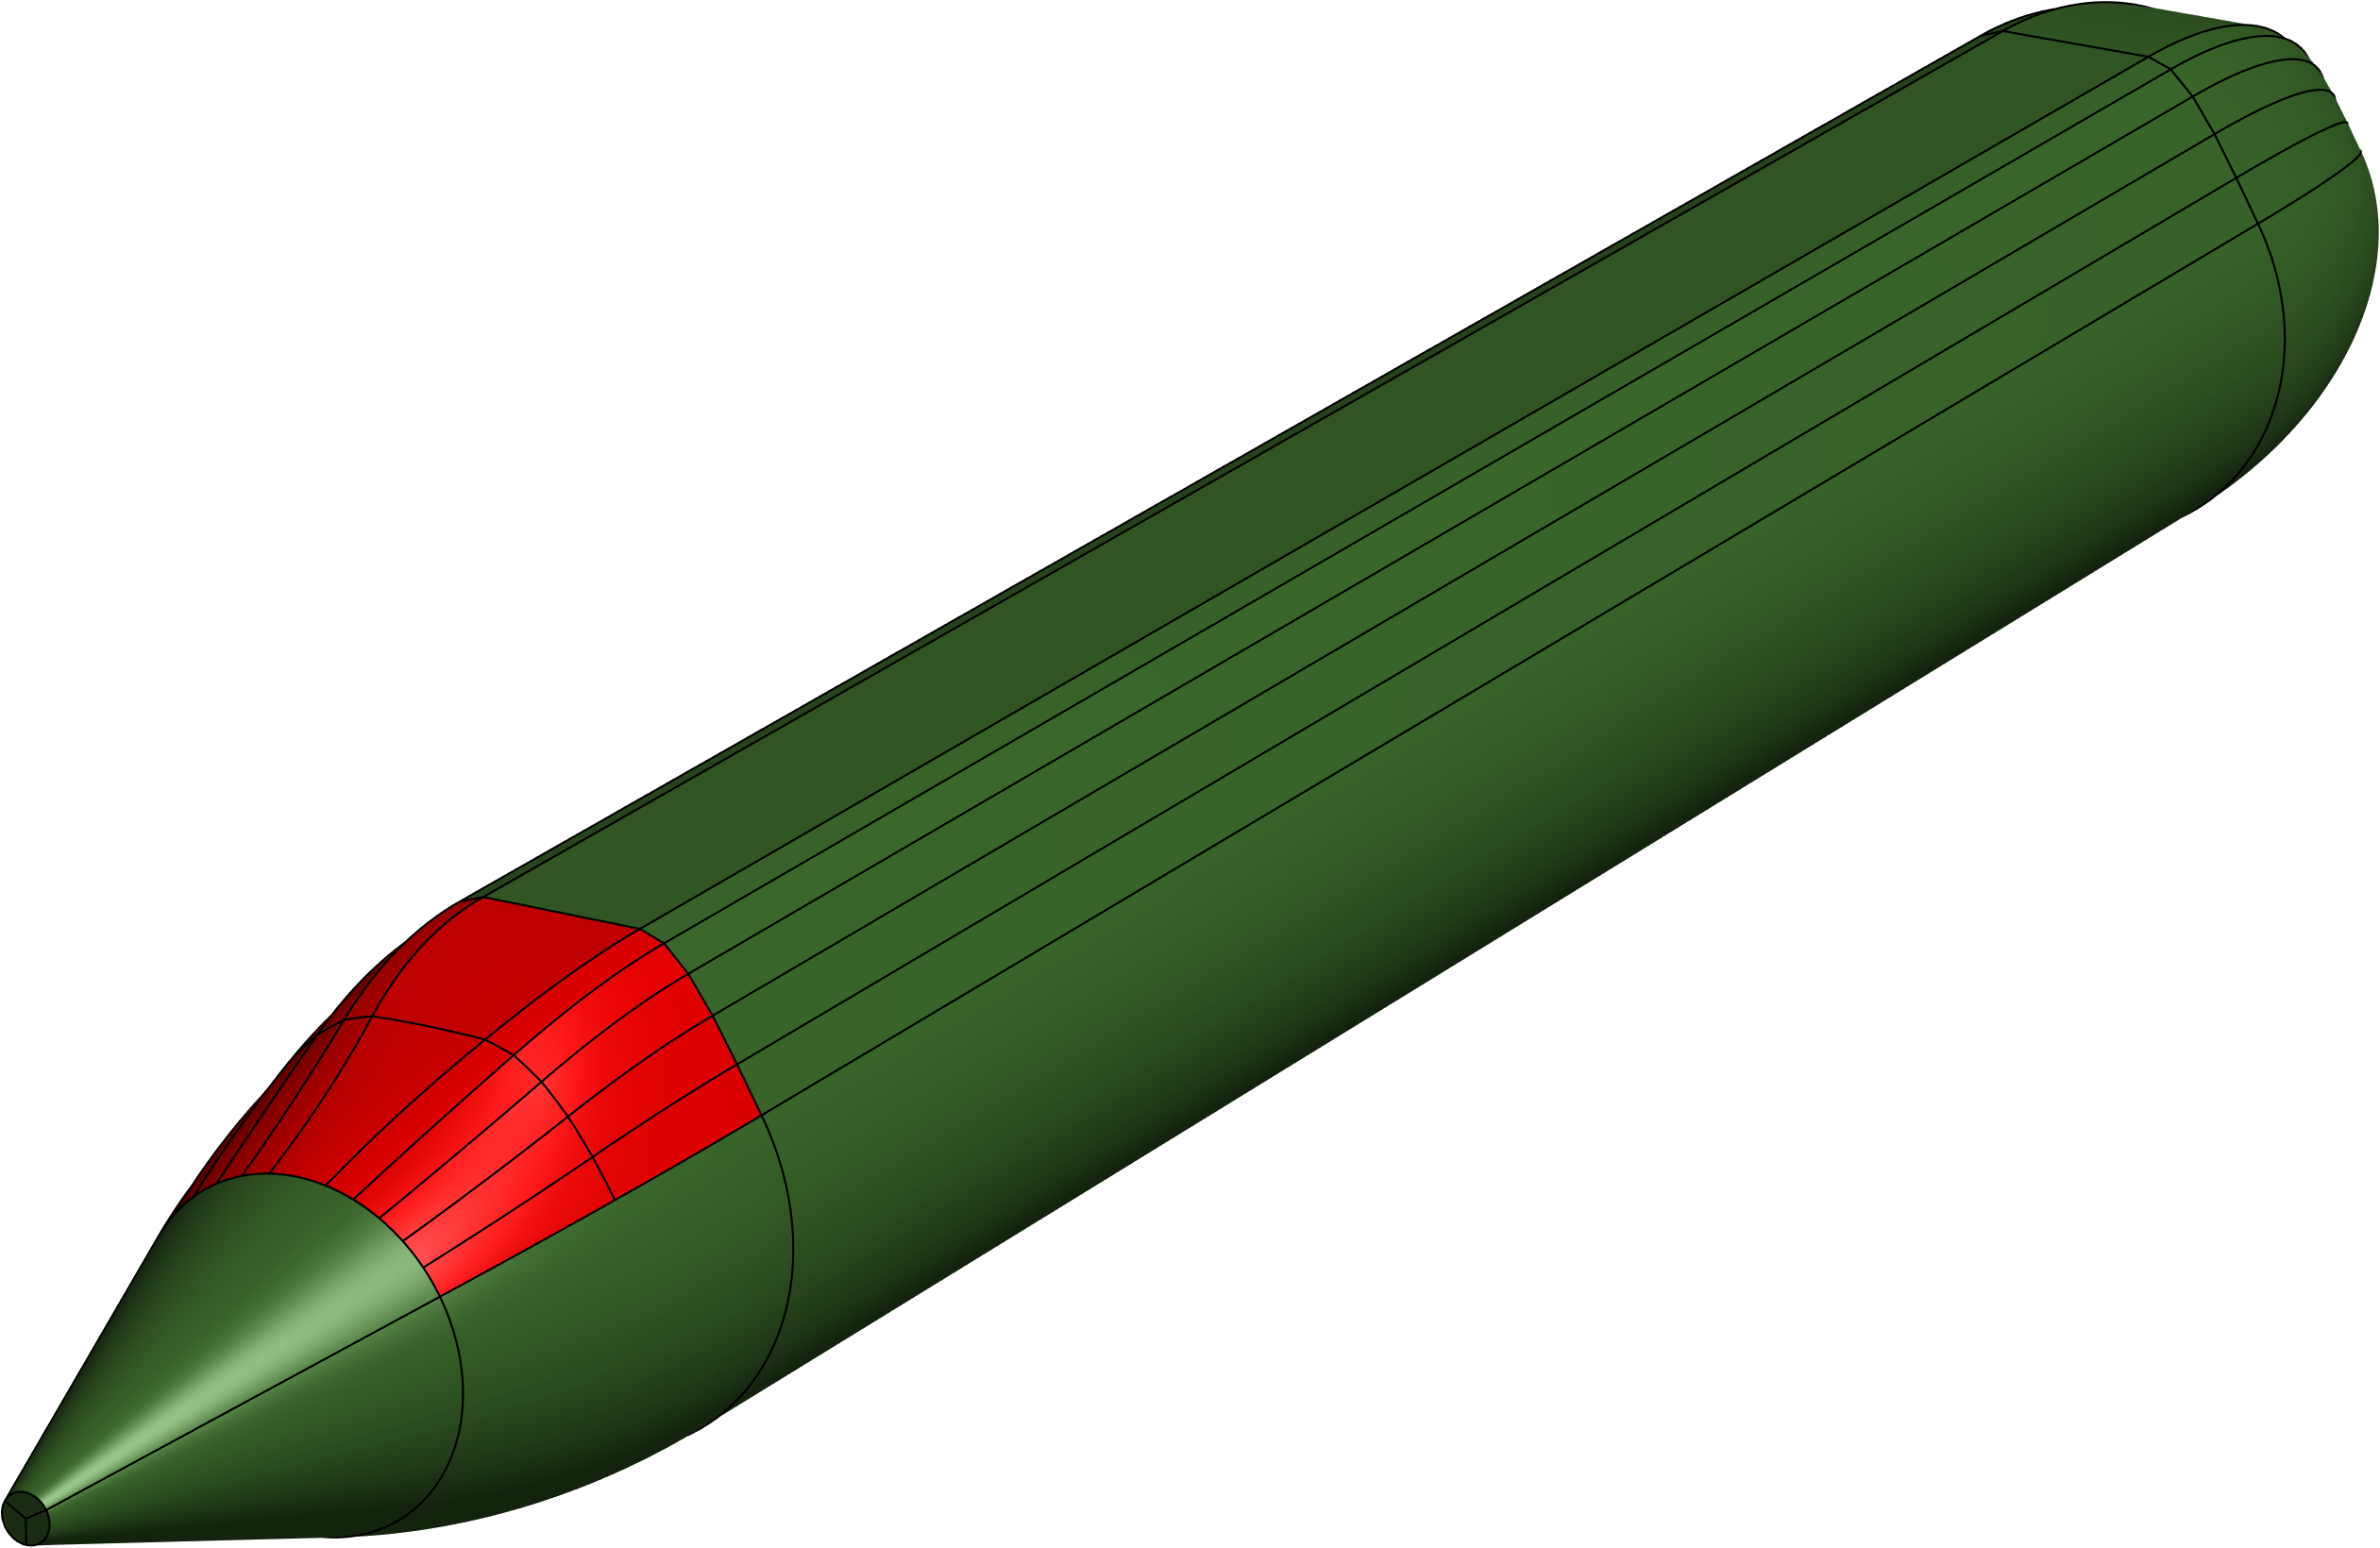
\includegraphics[width=\textwidth]{BeTSSi_BCpart3}
		\caption{Illustration of upper transition part.}
		\label{Fig2:bettsi_upperPartOfTailSection}
	\end{subfigure}
	\caption{Final patches for the stripped BeTSSi submarine.}
\end{figure}
As illustrated in \Cref{Fig2:BeTSSi_BC_tailSection}, the NURBS patch is given by 22 elements. Thus, $4\cdot 23 = 92$ control points, $\vec{P}_{i,j}$, is needed as shown in \Cref{Fig2:BeTSSi_BC_tailSection_cp} (23 and 4 control points in the $\xi$ direction and $\eta$ direction, respectively).
\begin{figure}
	\centering    
	\begin{subfigure}{0.49\textwidth}
		\centering
		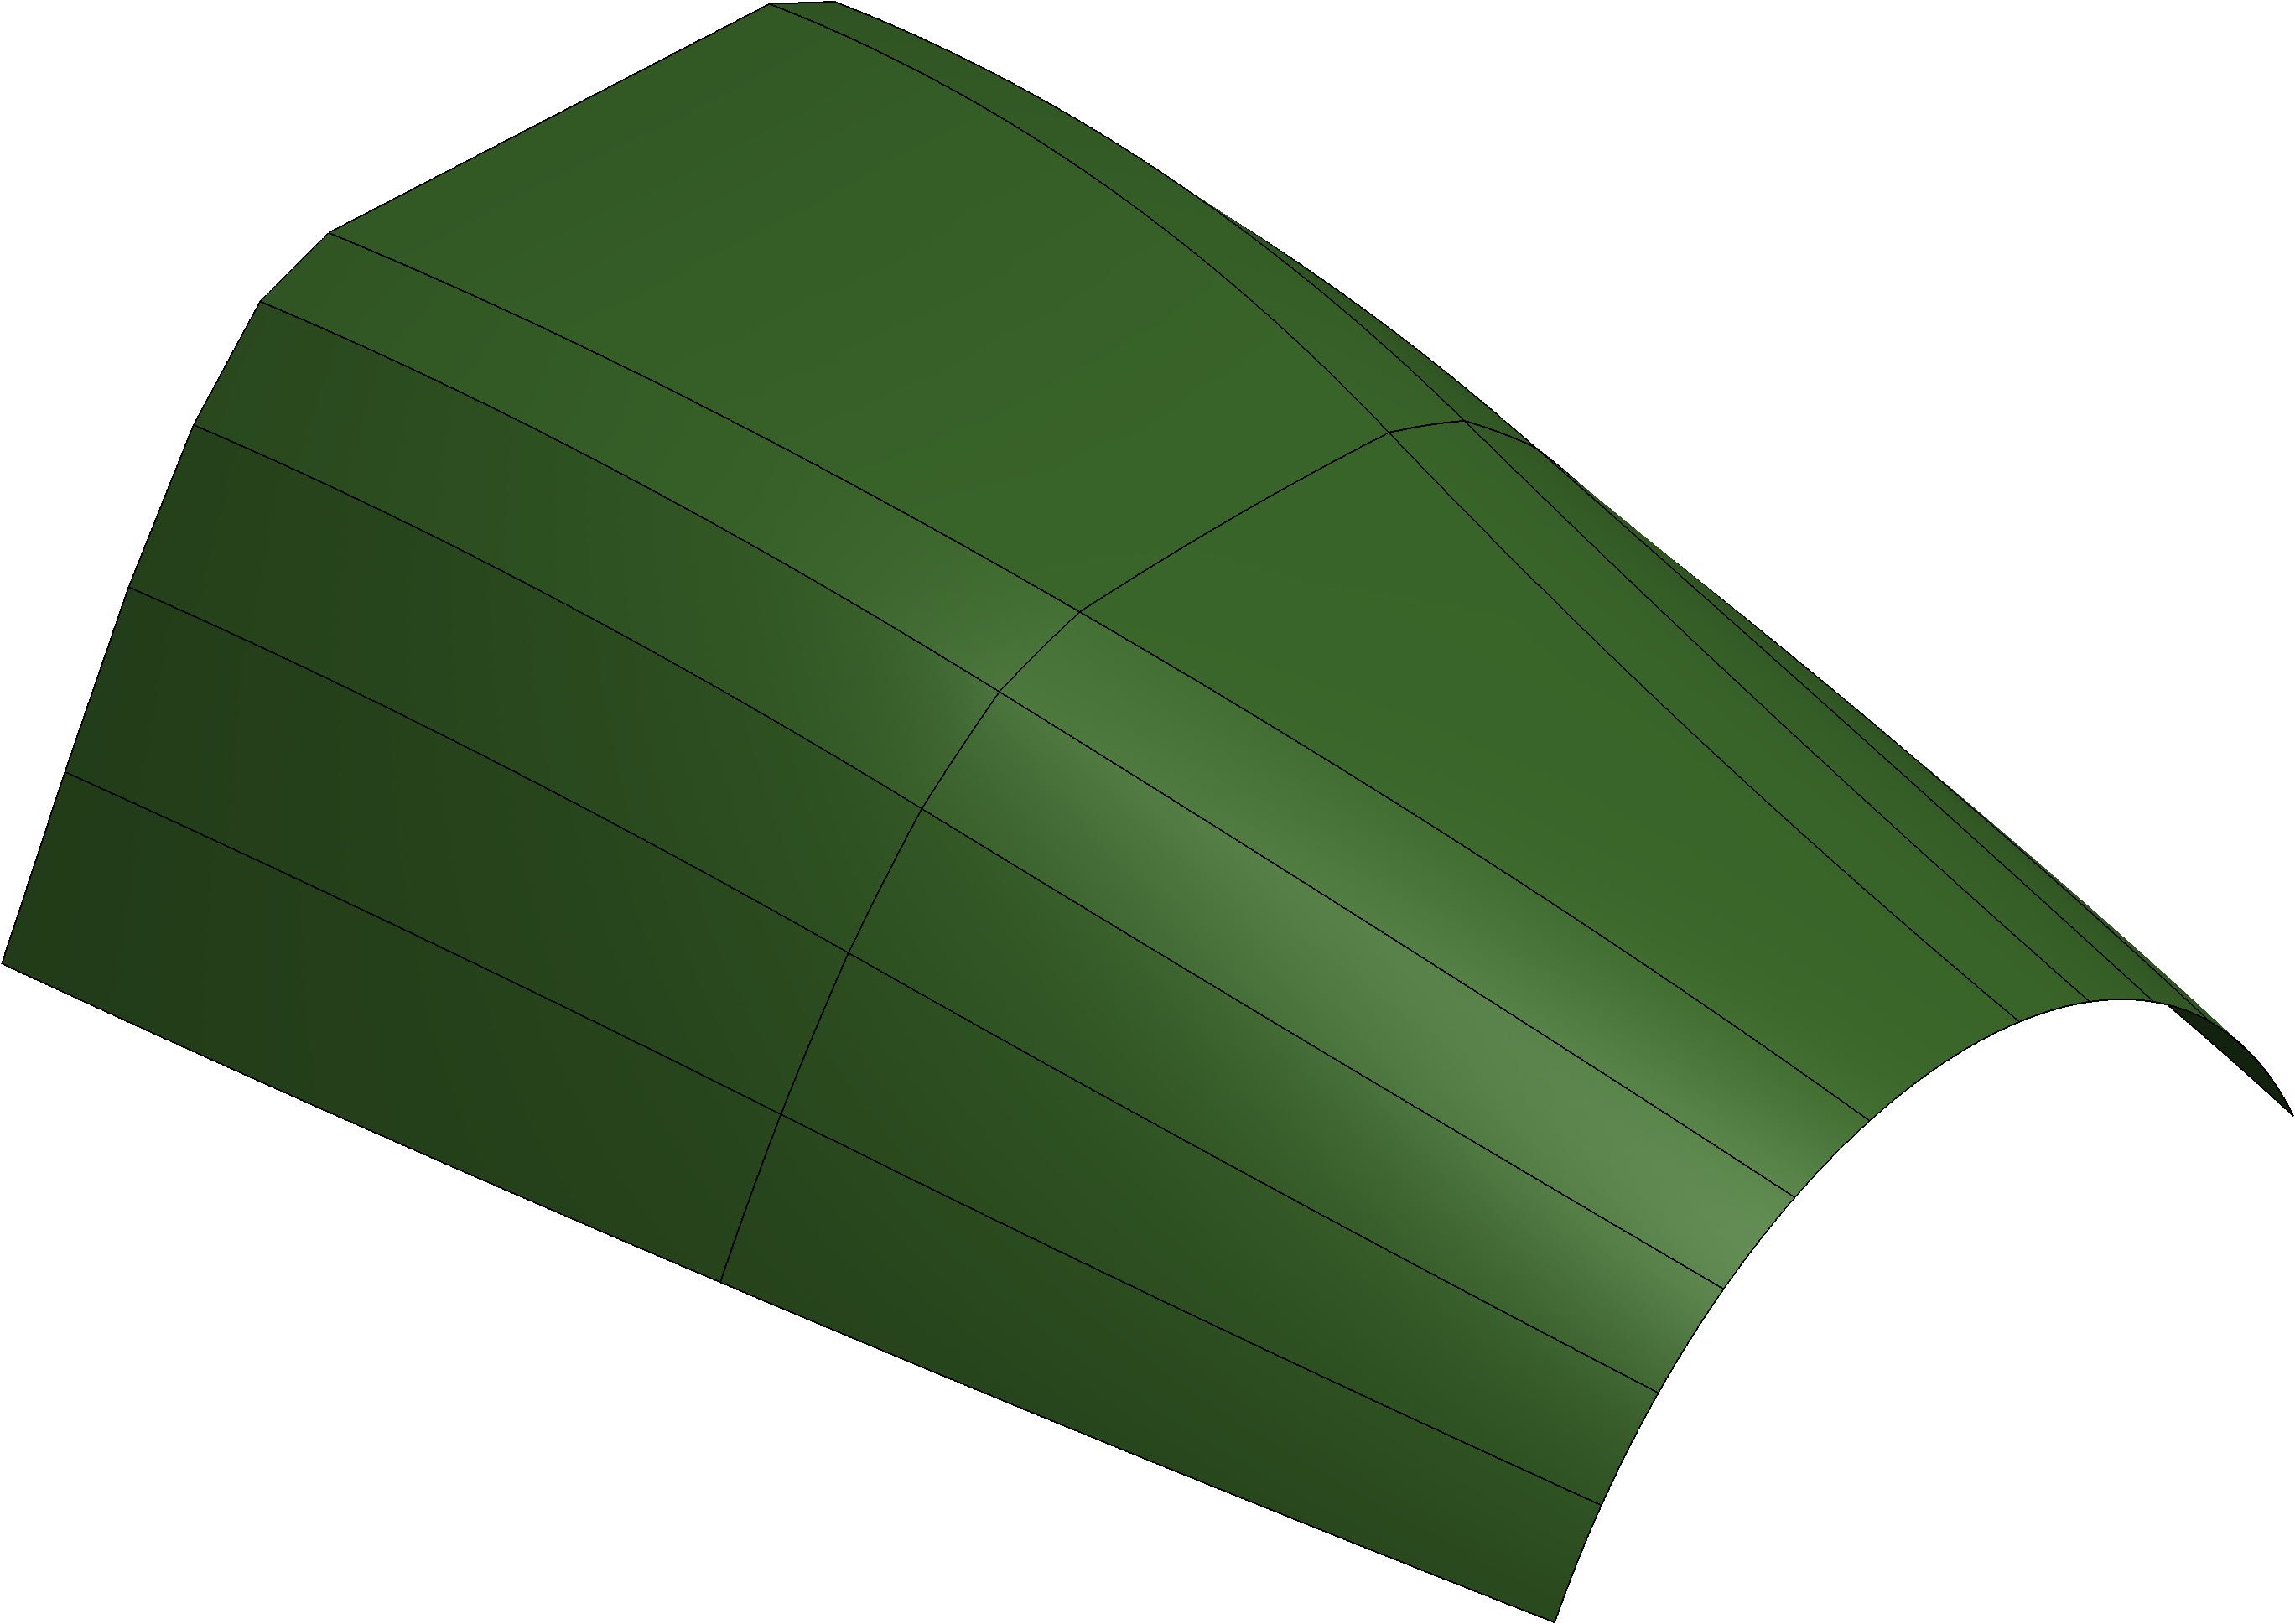
\includegraphics[width=0.9\textwidth]{BeTSSi_BC_tailSection}
		\caption{Illustration of the mesh.}
		\label{Fig2:BeTSSi_BC_tailSection}
	\end{subfigure}%
	\hspace*{0.02\textwidth}%   
	\begin{subfigure}{0.49\textwidth}
		\centering
		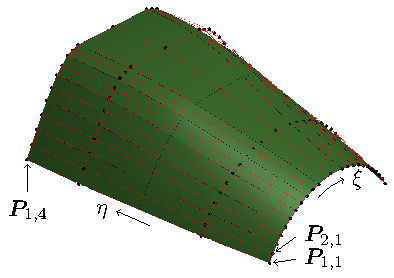
\includegraphics{tailSection}
		\caption{Illustration of the control polygon mesh.}
		\label{Fig2:BeTSSi_BC_tailSection_cp}
	\end{subfigure}
	\caption{Illustration of the upper transition part of the tail.}
\end{figure}
The control points $\vec{P}_{1,j}$ and $\vec{P}_{23,j}$ for $j=1,2,3,4$ must be defined as in \Cref{Fig2:arcParam2}, while the control points $\vec{P}_{i,1}$ must be defined as in \Cref{Fig2:arcParam1} (with corresponding weights). For $2\leq i\leq 22$ the weights are defined by $w_{i,j}=w_{i,1}$ for $j=2,3,4$. That is,
\begin{equation}
	w_{i,j} = \begin{cases}
		1 & i\,\, \text{odd}\\
		\cos\left(\frac{2\PI-\beta}{24}\right) & i\,\, \text{even},\,i\neq 12\\
		\cos\left(\frac{2\PI-\beta}{12}\right) &  i = 12
		\end{cases}		
\end{equation}
The location of the control points $\vec{P}_{i,j}$, $j=2,3$ and $2\leq i\leq 22$, are determined by the requirement that the $x$ component is the same as $\vec{P}_{1,j}$ and the fact that the control polygon lines must be tangential to the surface both at the deck and the cone tail.
\begin{figure}
	\centering    
	\begin{subfigure}[t]{0.44\textwidth}
		\centering
		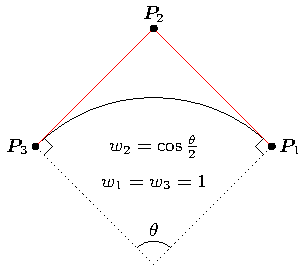
\includegraphics{knotInsertionArc_1}
		\caption{NURBS parametrization of arc of angle $\theta$ using three control points $\{\vec{P}_i\}_{i=1}^3$, the weights $\{w_i\}_{i=1}^3$ and the open knot vector $\Xi=\{0,0,0,1,1,1\}$.}
		\label{Fig2:arcParam1}
	\end{subfigure}%
	\hspace*{0.02\textwidth}%
	\begin{subfigure}[t]{0.54\textwidth}
		\centering
		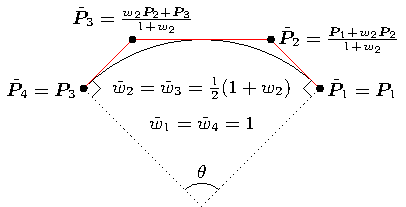
\includegraphics{knotInsertionArc_2}
		\caption{NURBS parametrization of arc of angle $\theta$ using four control points $\{\tilde{\vec{P}}_i\}_{i=1}^4$, the weights $\{\tilde{w}_i\}_{i=1}^4$ and the open knot vector $\tilde{\vec{t}}_\upxi=\{0,0,0,0.5,1,1,1\}$.}
		\label{Fig2:arcParam2}
	\end{subfigure}%
	\caption{Two ways of parametrizing an arc using NURBS~\cite[p. 315]{Piegl1997tnb}.}
\end{figure}

The inner surface of the BeTSSi submarine is generated by scaling a copy of the outer surface with the following change in the parameters $a\to a-t$, $b\to b-t$, $c\to c-t$, $s\to s-t/2$,  $g_2\to g_2-t/2$ and $g_3\to g_3-t/2$ ($\alpha$, $\beta$ and $l$ remain unchanged).